\documentclass[conference]{IEEEtran}
\IEEEoverridecommandlockouts
% The preceding line is only needed to identify funding in the first footnote. If that is unneeded, please comment it out.
%Template version as of 6/27/2024

% ##### THIS IS IEEE INCLUDED ###################

\usepackage{cite}
\usepackage{amsmath,amssymb,amsfonts}
\usepackage{algorithmic}
\usepackage{graphicx}
\usepackage{textcomp}
\usepackage{xcolor}
\def\BibTeX{{\rm B\kern-.05em{\sc i\kern-.025em b}\kern-.08em
    T\kern-.1667em\lower.7ex\hbox{E}\kern-.125emX}}

% ##############################################

% ##### THIS IS MY INCLUDED ###################

\usepackage{cleveref} % For referencing

% ##############################################

\begin{document}

\title{Conference Paper Title*\\
    % {\footnotesize \textsuperscript{*}Note: Sub-titles are not captured for https://ieeexplore.ieee.org  and
    % should not be used}
    % \thanks{Identify applicable funding agency here. If none, delete this.}
}

% ##############################################

% Use \textit for university names
% Use \texttt for email addresses
% Use Mark with \IEEEauthorrefmark{1} for seperate information
% Use one block for same university
% Use { } for email when end is same. Example: {abc,xyz}@gmail.com

% ##############################################

% \author{\IEEEauthorblockN{1\textsuperscript{st} Given Name Surname}
%     \IEEEauthorblockA{\textit{dept. name of organization (of Aff.)} \\
%         \textit{name of organization (of Aff.)}\\
%         City, Country \\
%         email address or ORCID}
%     \and
%     \IEEEauthorblockN{2\textsuperscript{nd} Given Name Surname}
%     \IEEEauthorblockA{\textit{dept. name of organization (of Aff.)} \\
%         \textit{name of organization (of Aff.)}\\
%         City, Country \\
%         email address or ORCID}
%     \and
%     \IEEEauthorblockN{3\textsuperscript{rd} Given Name Surname}
%     \IEEEauthorblockA{\textit{dept. name of organization (of Aff.)} \\
%         \textit{name of organization (of Aff.)}\\
%         City, Country \\
%         email address or ORCID}
%     \and
%     \IEEEauthorblockN{4\textsuperscript{th} Given Name Surname}
%     \IEEEauthorblockA{\textit{dept. name of organization (of Aff.)} \\
%         \textit{name of organization (of Aff.)}\\
%         City, Country \\
%         email address or ORCID}
%     \and
%     \IEEEauthorblockN{5\textsuperscript{th} Given Name Surname}
%     \IEEEauthorblockA{\textit{dept. name of organization (of Aff.)} \\
%         \textit{name of organization (of Aff.)}\\
%         City, Country \\
%         email address or ORCID}
%     \and
%     \IEEEauthorblockN{6\textsuperscript{th} Given Name Surname}
%     \IEEEauthorblockA{\textit{dept. name of organization (of Aff.)} \\
%         \textit{name of organization (of Aff.)}\\
%         City, Country \\
%         email address or ORCID}
% }

\author{
    \IEEEauthorblockN{
        Michael Shell\IEEEauthorrefmark{1},
        Homer Simpson\IEEEauthorrefmark{2},
        James Kirk\IEEEauthorrefmark{3},
        Montgomery Scott\IEEEauthorrefmark{3}
        and Eldon Tyrell\IEEEauthorrefmark{4}
    }
    \IEEEauthorblockA{
        \IEEEauthorrefmark{1}School of Electrical and Computer Engineering\\
        Georgia Institute of Technology, Atlanta, Georgia 30332--0250\\
        Email: mshell@ece.gatech.edu
    }
    \IEEEauthorblockA{
        \IEEEauthorrefmark{2}Twentieth Century Fox, Springfield, USA\\
        Email: homer@thesimpsons.com
    }
    \IEEEauthorblockA{
        \IEEEauthorrefmark{3}Starfleet Academy, San Francisco, California 96678-2391\\
        Telephone: (800) 555--1212, Fax: (888) 555--1212
    }
    \IEEEauthorblockA{
        \IEEEauthorrefmark{4}Tyrell Inc., 123 Replicant Street, Los Angeles, California 90210--4321
    }
}

\maketitle

\begin{abstract}
    This document is a model and instructions for \LaTeX.
    This and the IEEEtran.cls file define the components of your paper [title, text, heads, etc.]. *CRITICAL: Do Not Use Symbols, Special Characters, Footnotes,
    or Math in Paper Title or Abstract.
\end{abstract}


\begin{IEEEkeywords}
    component, formatting, style, styling, insert.
\end{IEEEkeywords}

\section{Introduction}
\label{sec:introduction}

This is the introduction section. PLEASE EDIT. \cite{IEEEexample:bluebookbook}

\subsection{Sub Sections}
\label{subsec:subsections1}

This is the sub section of the introduction. PLEASE EDIT.


\section{Related Works}
\label{sec:relatedworks}

This is the related works section. PLEASE EDIT.

\section{System Overview}
\label{systemoverview}

This is the system overview section. PLEASE EDIT.

\section{Design and Development}
\label{sec:designanddevelopment}

This is the design and development section. PLEASE EDIT.

\section{Result and Discussion}
\label{resultsanddiscussion}

This is the result and discussion section. PLEASE EDIT.

\section{Conclusion}
\label{sec:conclusion}

This is the conclusion section. PLEASE EDIT.

This is cite example. \cite{IEEEexample:bluebookbook}

This is reference. \cref{conclusion,designanddevelopment} or \ref{introduction}
\newline
\begin{itemize}
    \item Use either SI (MKS) or CGS as primary units. (SI units are encouraged.) English units may be used as secondary units (in parentheses). An exception would be the use of English units as identifiers in trade, such as ``3.5-inch disk drive''.
    \item Avoid combining SI and CGS units, such as current in amperes and magnetic field in oersteds. This often leads to confusion because equations do not balance dimensionally. If you must use mixed units, clearly state the units for each quantity that you use in an equation.
    \item Do not mix complete spellings and abbreviations of units: ``Wb/m\textsuperscript{2}'' or ``webers per square meter'', not ``webers/m\textsuperscript{2}''. Spell out units when they appear in text: ``. . . a few henries'', not ``. . . a few H''.
    \item Use a zero before decimal points: ``0.25'', not ``.25''. Use ``cm\textsuperscript{3}'', not ``cc''.)
\end{itemize}

\begin{equation}
    a+b=\gamma\label{eq}
\end{equation}

\begin{table}[htbp]
    \caption{Table Type Styles}
    \begin{center}
        \begin{tabular}{|c|c|c|c|}
            \hline
            \textbf{Table} & \multicolumn{3}{|c|}{\textbf{Table Column Head}}                                                         \\
            \cline{2-4}
            \textbf{Head}  & \textbf{\textit{Table column subhead}}           & \textbf{\textit{Subhead}} & \textbf{\textit{Subhead}} \\
            \hline
            copy           & More table copy$^{\mathrm{a}}$                   &                           &                           \\
            \hline
            \multicolumn{4}{l}{$^{\mathrm{a}}$Sample of a Table footnote.}
        \end{tabular}
        \label{tab1}
    \end{center}
\end{table}

\begin{figure}[htbp]
    \centerline{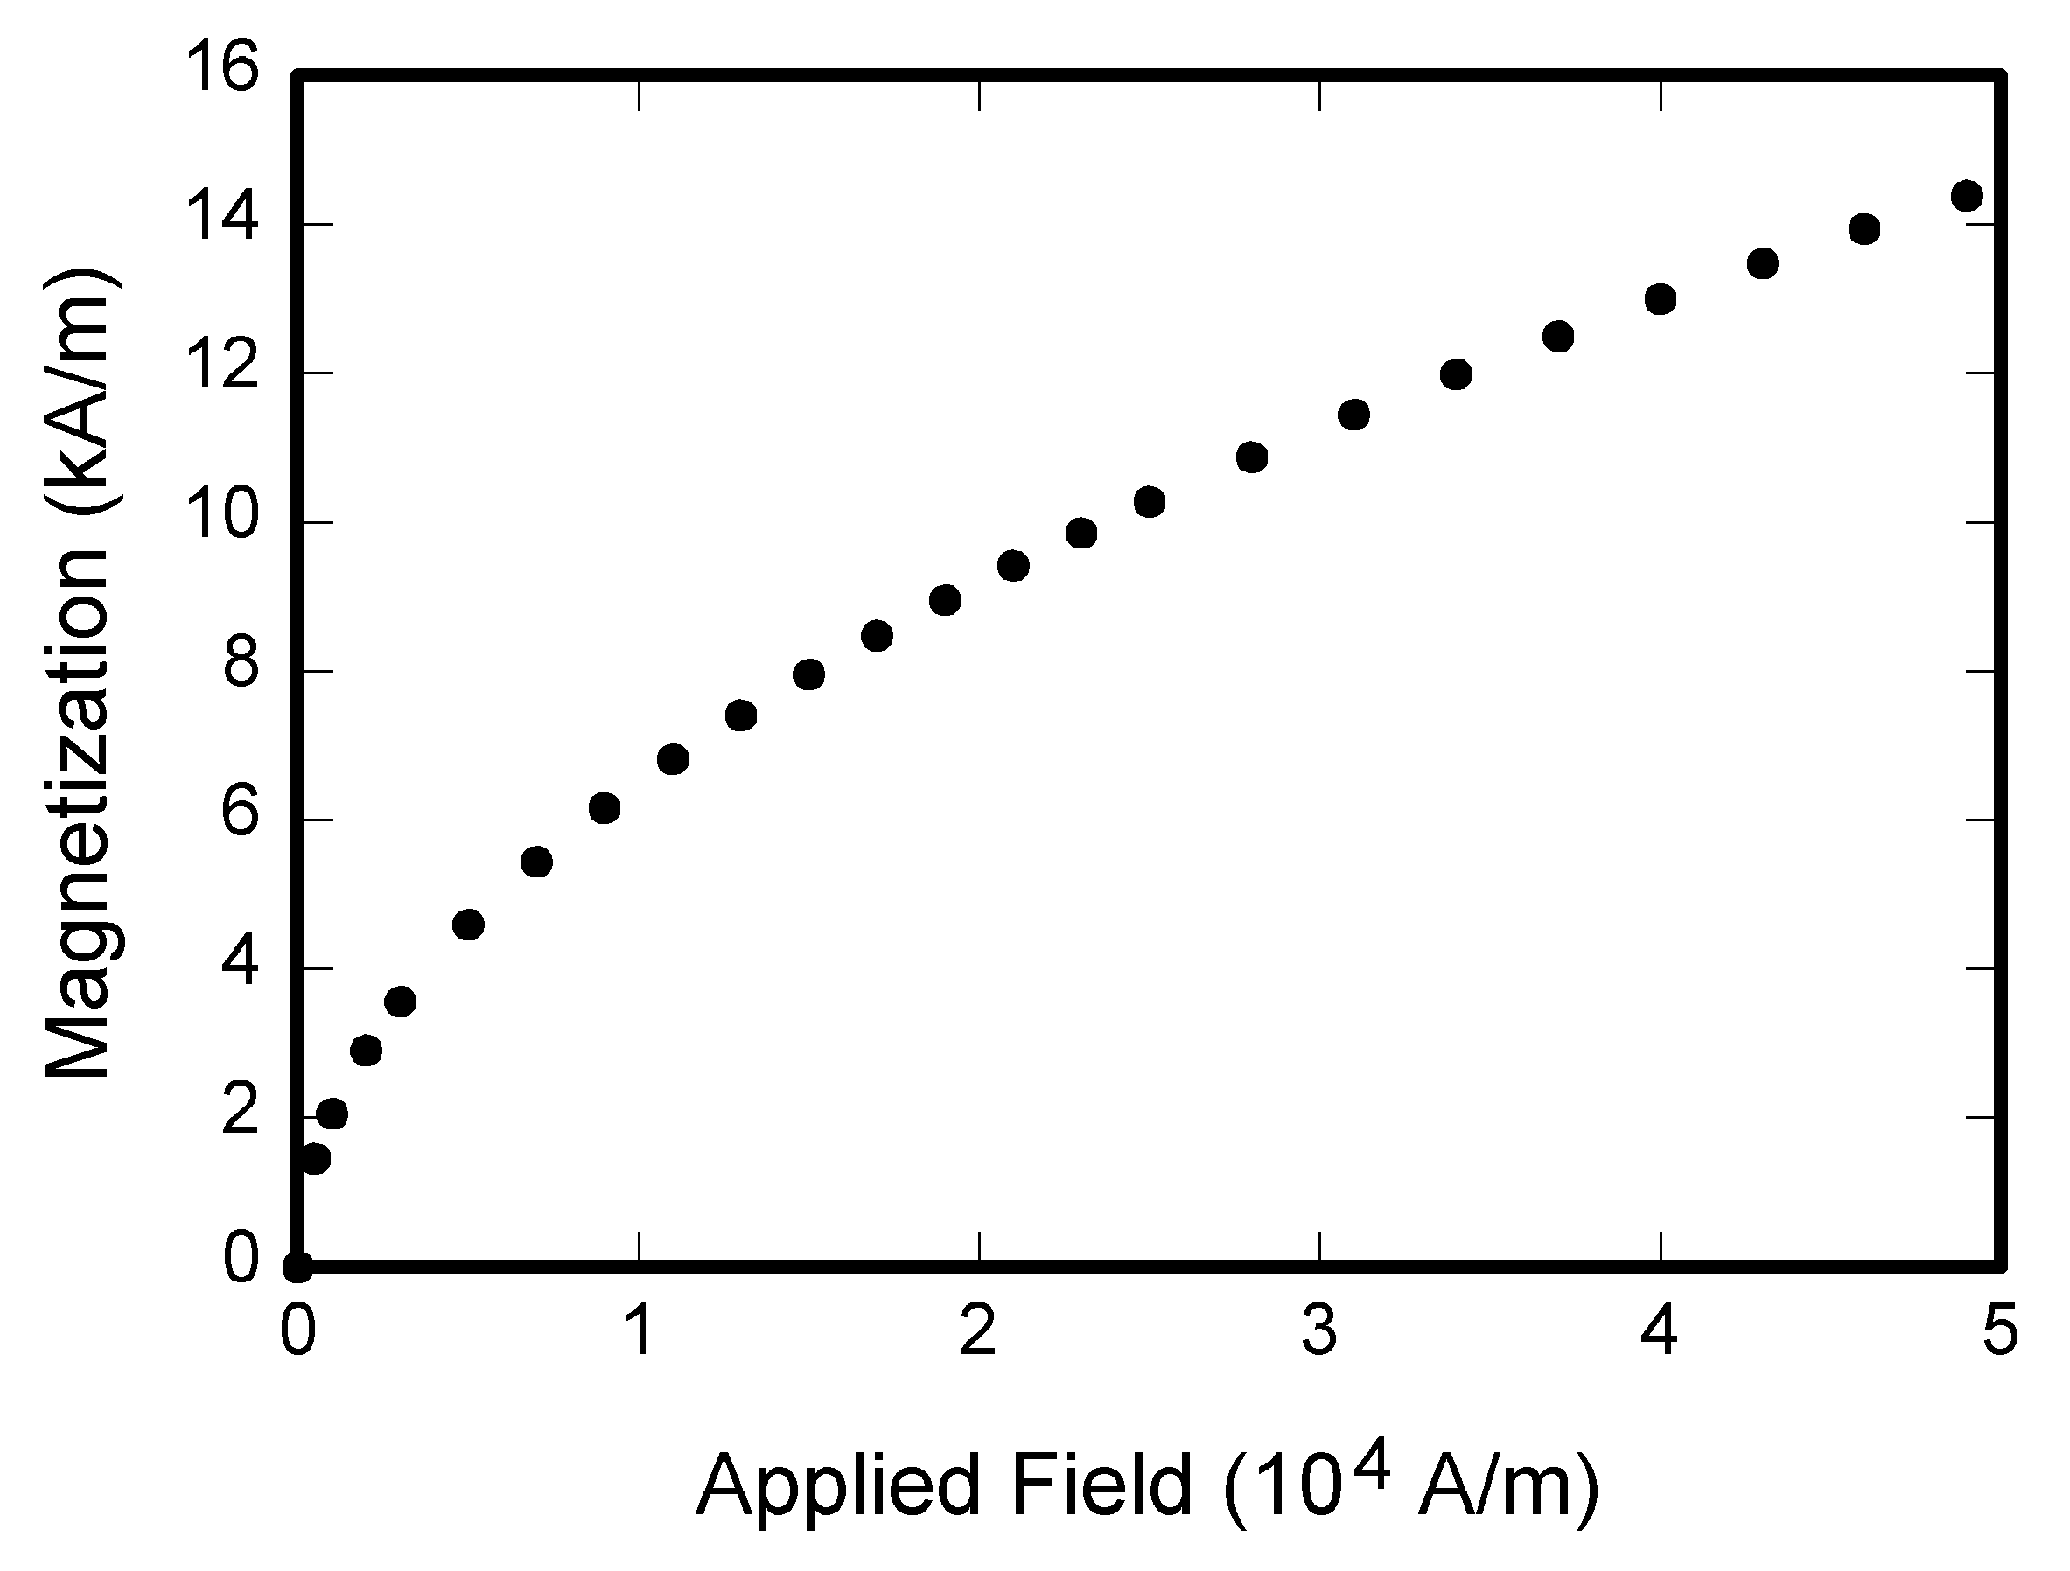
\includegraphics[width=0.5\textwidth]{Photos/fig1.png}}
    \caption{Example of a figure caption.}
    \label{fig}
\end{figure}

\bibliographystyle{IEEE_Files/IEEEtran}
\bibliography{reference}


\end{document}
